\documentclass{article}
\usepackage[utf8]{inputenc}
\usepackage[]{hyperref}

\author{
  Raatikka, Marko\\
  \texttt{marko.raatikka@aalto.fi}
  \and
  Lucas, Triefenbach\\
  \texttt{lucas.triefenbach@aalto.fi}
}
\title{Energy efficiency of HTTP2 over HTTP1.1 on the mobile web
\\
\vspace{5mm}
\large{CSE-E5440: Energy-efficient Mobile Computing\\Group C}
}
\date{\today}

\usepackage{natbib}
\usepackage{graphicx}

\begin{document}

\maketitle
\clearpage

\section{Part I}

\subsection{Introduction}
With the increasing computation power and connection speed of mobile phones in recent years, the amount of data flowing through the Internet to the consumer's end device continues to grow. While web applications have become ever more complex and the amount of HTML, JavaScript and CSS required to render a web page has grown, HTTP1.1 -- the prevailing transfer protocol of today's web -- has failed to keep up with the pace. One of the culprits of HTTP1.1 is that it can only handle one request per a TCP connection and that it can only have a certain maximum number of connections per host (5-8 connections depending on the browser). To work around these shortcomings developers have used techniques such as domain sharding (hosting assets across multiple domains), image spriting and inlining CSS \& JavaScript. However, a transport layer problem can not be efficiently solved at the application level.

The work for a new version of HTTP protocol was set forth by Google in 2012 in the form an open networking protocol called SPDY. Later, in 2015 , building on the work done for SPDY, HTTP2 was proposed as the future standard protocol. The biggest improvements HTTP2 introduces over HTTP1.1 are multiplexing of requests and responses to avoid a so called \emph{head-of-line blocking} inherent in HTTP1, header compression, prioritization of requests and server push mechanism. Web services are slowly migrating into adopting HTTP2, but as of today, only about 7\% of the websites have fully migrated to the new protocol. \citep{google-spdy}\citep{http2_stats}\citep{http2}

This work sets to study the impact of HTTP2 on mobile power consumption. Previous work on the topic has been done by \citep{previous_work}. However, this work focuses more on generating high traffic and mimicking common navigation patterns. Due to time constraints testing is limited to a single browser as opposed to testing across various versions. The content is organized as follows: chapter \ref{chapter:design-implementation} describes the method used, the testbed environment and the steps of a test run. Chapter \ref{chapter:results} continues by presenting the experiment results, which are later reviewed in Chapter \ref{chapter:discussion}. Last, an outline for the part II of the study is given.


\subsection{Design and Implementation}
\label{chapter:design-implementation}

The energy efficiency of the HTTP1.1 and HTTP2 protocols were measured by generating large amounts of network traffic. Six different web services were chosen as the targets, including Flickr, Yahoo, Facebook, Twitter, Weather.com and Instagram. These web services were selected based on their popularity and support for HTTP2 clients (browsers). Facebook, Twitter and Weather.com were eventually omitted from the final experiment corpus: the network traffic generated by Facebook was highly optimized, and therefore, it was assumed that it would not introduce any interesting differences in the payload sizes. Twitter on the other hand was deemed too lightweight (consisting of mostly text-based content), while Weather.com suffered from peculiar latency issues when transmitting images over HTTP2 as shown by Figure \ref{fig:weather.com}.

\begin{figure}[h!]
\centering
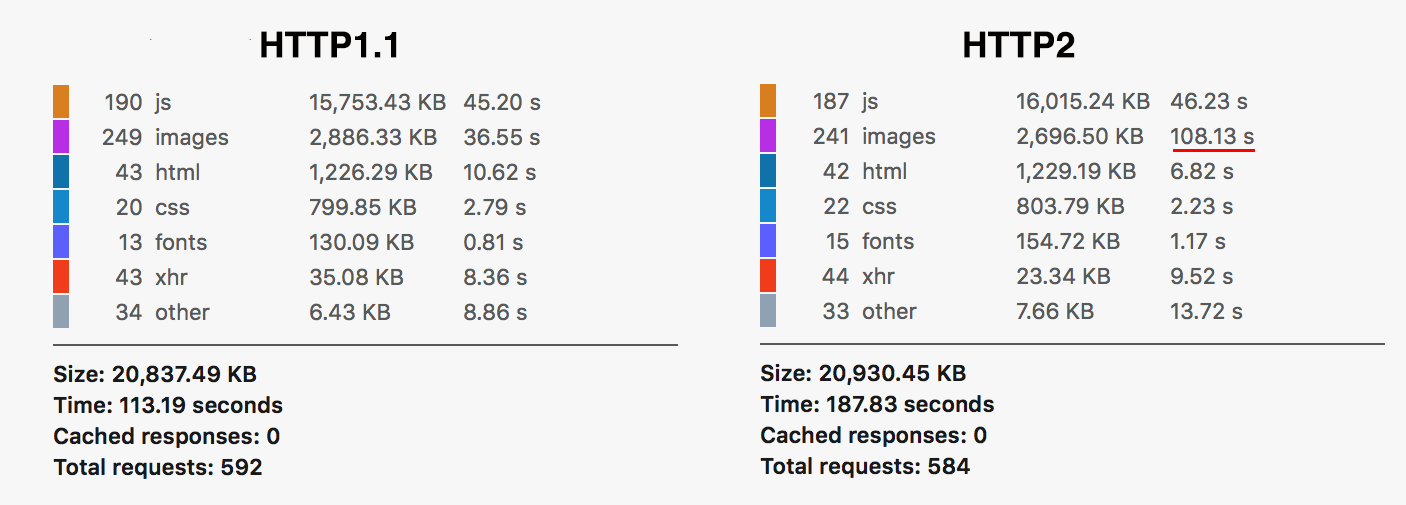
\includegraphics[scale=0.6]{weathercom.png}
\caption{Weather.com was excluded from the final experiment corpus because it exhibited abnormally long response times when image assets were fetched over HTTP2. This was done the prevent introducing bias to the energy consumption measurements.}
\label{fig:weather.com}
\end{figure}

The experiment was conducted using Firefox (version 42.0) as no other publicly available browsers support manually disabling HTTP2 support, as of this writing. The implementation of a robust and reproducible experiment environment required automation of the navigation logic. Browser automation frameworks Appium\footnote{Appium - \url{appium.io}} and Mozilla’s Robocop\footnote{Robocop - \url{https://wiki.mozilla.org/Auto-tools/Projects/Robocop}} were originally considered for this task. However, Appium lacked support for the Firefox browser, and Robocop -- Mozilla’s internal tool for testing Firefox on mobile -- missed proper documentation. Thus, an alternative approach -- including the use of Android’s low level input API -- was taken. The utilization of the input API was inspired by an open-source energy consumption measurement framework called GreenMiner \citep{greenminer}.

The Android input API allows for the emulation of device gestures, and consequently, automation of browser navigation. The trade-off of this approach is that it requires root access to the device. Therefore the Samsung S4 used for the experiment was rooted using ClockworkMod recovery (version 6.0.4.7) and CyanogenMod (version 12), which ships with Android 5.1.1. The upside of installing a custom ROM -- a customized OS image installed on the device's ROM memory -- like CyanogenMod is that any pre-installed Google services or bundled Samsung software were not installed in the phone. This helped in minimizing any unwanted power consumption generated by services running in the background unknowingly.

Monsoon Solutions' Power Monitor\footnote{\url{https://www.msoon.com/LabEquipment/PowerMonitor/}} was used for collecting the power consumption data. The negative and positive terminals of the smartphone battery were connected to the power monitor using copper wire. The two reading terminals of the Samsung S4 battery were isolated to allow the smartphone to be started using external power (the power monitor). Output voltage set to 3.7V as per Samsung S4 battery information.

For the test setup most smartphone features were disabled. This ,includes automatic brightness, notifications, sounds, vibrations, locking of the screen and even battery information. The only main features enabled were wifi, airplane mode and developer mode. Further the screen was set to maximum brightness.
So basically only the debugging via adb and networking via wifi was activated.
Wifi is the only type of networking used in the setup for the following reason.
Different types of connections were tested and in the testing location 2G resulted in a high paket loss, which made 2G incomparable to the other types. While 3G and 4G did not display any difference in latency and package loss, than the wifi connected to the aalto-open network. This may be due to the setup station being located near the mobile providers antennas, which are on the roof of the CS building. For this reason only wifi was used in the testing setup. Another factor that might have an influence on the latency is that all readings were taken in the evening, when the building was nearly empty. This results in low latency, since all networks have low loads in general. On the other hand testig during the day might lead to biased results because of higher load fluctuations in the networks.


test setup (testbed environment)
    disable some smartphone features
    disable browser features (caching)
    network environment (why WiFi and not 2G, 3G, latency table in Google Drive)
    sampling frequency 5000Hz

test run procedure
    steps
    duration

list relevant test variable values


\subsection{Results}
\label{chapter:results}

RESULTS
    baseline power OS: 1 W \\
    app baseline power with Browser: 1.8 W \\
    mean power consumption +- stdev
    smoothed graph (3 runs for both)
    "aggregated" graph (average of every 1s segment (5000samples))
        annotation
    network request pie chart

\begin{figure}[h!]
\centering
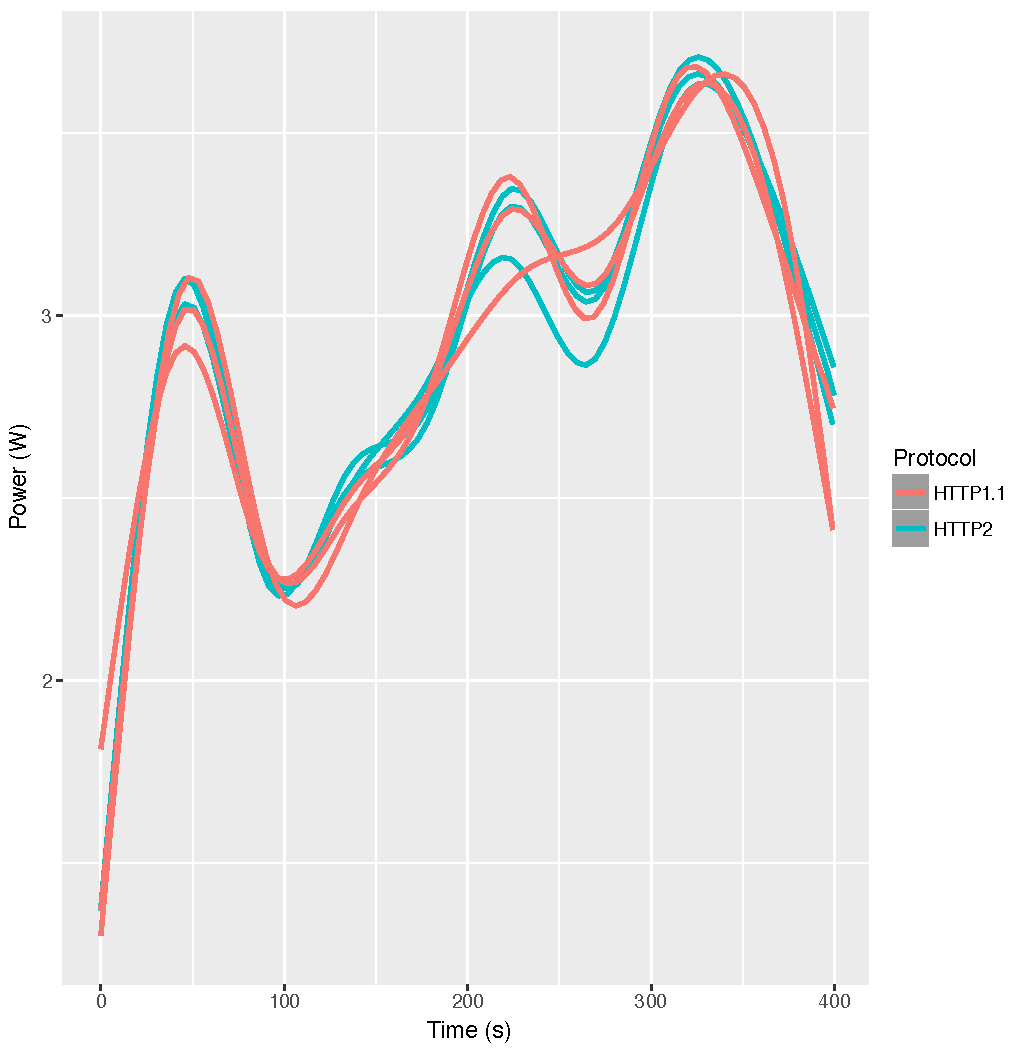
\includegraphics[scale=0.7]{smoothed_power}
\caption{smoothed out power levels of all test runs in HTTP2 and HTTP1 }
\label{fig:smoothed_power}
\end{figure}

\begin{figure}[h!]
\centering
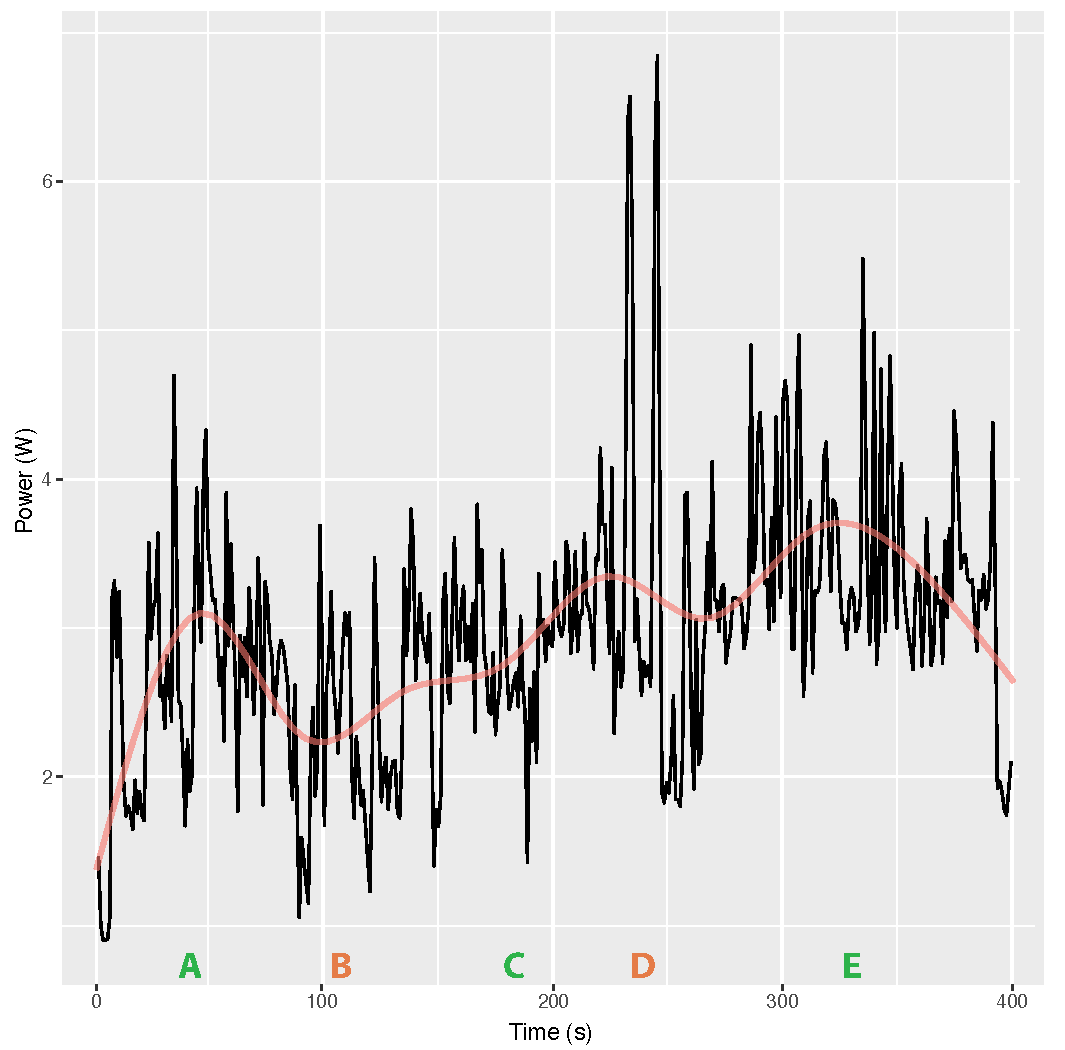
\includegraphics[scale=0.675]{average_power}
\caption{Reading of power levels compared to smoothed out readings in a HTTP/1.1 example}
\label{fig:average_power}
\end{figure}

\begin{table}[]
    \centering
    \begin{tabular}{c|c|c}
        & \textbf{HTTP1.1} & \textbf{HTTP2}  \\
        Mean (W)   & 2.987 & 2.995 \\
        Std.dev (W) & 0.984 & 1.007 \\
        Total (J)  & 1114.2 & 1117.2 \\
    \end{tabular}
    \caption{Energy consumption of HTTP1.1 and HTTP2}
    \label{table:energy_consumption}
\end{table}


\begin{table}[]
    \centering
    \begin{tabular}{c|c|c|c}
         \textbf{Web service} & \textbf{RTT (ms)} & \textbf{RTT std. dev (ms)} & \textbf{Packet loss} \\
        Yahoo   & 158 & 32 & 4.7\% \\
        Instagram  & 116 & 10 & 0.3\% \\
        Flickr & 132 & 12 & 0.3\% \\
    \end{tabular}
    \caption{Latency of our websites}
    \label{table:latency}
\end{table}



\begin{figure}[h!]
\centering
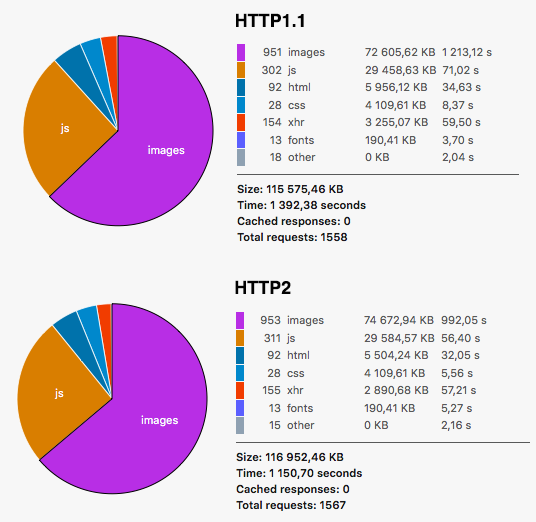
\includegraphics[scale=0.6]{http2_consumes.png}
\caption{The better latency of HTTP2 comes with the price of performance.}
\label{fig:weather.com}
\end{figure}

\subsection{Discussion}
\label{chapter:discussion}

DISCUSSION
    talk about ENERGISE (\url{https://github.com/ds4se/chapters/blob/master/abramhindle/energymining.md#Hindle2014})
    interpretation of results (explain A-E)
    outline for part II



\section{Part II}

\subsection{Proposal for Improvements}

\subsection{Conclusions}

\bibliographystyle{plain}
\bibliography{references}
\end{document}
